\documentclass[../main.tex]{subfiles}
%\newtheorem{theorem}{Stelling}
%\theoremstyle{definition}
%\newtheorem{definition}{Definitie}[section]

\begin{document}
\onlyinsubfile{
\setcounter{chapter}{3}
}
\notinsubfile{}

\section{Hilbertruimtes}\label{sec:POHilbert}


Aan het einde van de negentiende eeuw en in het begin van de twintigste eeuw werd er door veel wiskundige onderzoek gedaan naar abstracte vectorruimtes. Een van de mensen die dit onderzocht van David Hilbert (1862-1943), hij was zeer geïnteresseerd in zogenoemde $L^p$-ruimtes. Later heeft John von Neumann (1903-1957) zijn werk veralgemeniseerd naar abstracte vectorruimtes en heeft de Hilbertruimtes naar hem vernoemd.

Hilbertruimtes zijn belangrijk voor het begrijpen van quantumtheorie. Ze bieden een manier om op een abstractere manier over dingen te denken met behulp van vectoren. Zo kan je ze gebruiken om de "lengte" van een functies te berekenen of zelfs de stelling van Pythagoras te gebruiken voor functies.


\subsection*{Het standaard inproduct}
We beginnen met een korte herhaling van het al bekende inproduct. 
Voor twee vectoren in het vlak $x=(x_1,x_2)$ en $y=(y_1,y_2)$ is het standaard inproduct
\[x\cdot y =x_1y_1+x_2y_2\]
Op dezelfde manier kan je het inproduct nemen van twee $n$-dimensionale vectoren.
\[x\cdot y=x_1y_1+x_2y_2+\ldots+x_ny_n\]
Als twee vectoren loodrecht op elkaar staan dan is het inproduct 0, we zeggen dan dat de vectoren orthogonaal op elkaar staan.

Je kan de lengte van vector $x$ berekenen met het inproduct door $||x||=\sqrt{x\cdot x}$.

\begin{opdracht}
\begin{enumerate}
    \item Laat $x=\begin{pmatrix}-1\\4\\0\\2\end{pmatrix}$ en $y=\begin{pmatrix}0\\1\\-3\\2\end{pmatrix}$. Bereken $x\cdot y$.
    \item Ga na dat $(x+z)\cdot y=x\cdot y+ z\cdot y$.
    \item Vind twee vectoren die orthogonaal staan op $x=\begin{pmatrix}5\\-8\\0\end{pmatrix}$.
\end{enumerate}
\end{opdracht}
\subsection*{Het complexe geval}
Voor complexe vectoren kan je proberen het standaard inproduct op dezelfde manier te definiëren. Dit gaat mis omdat je lengtes krijgt die complex zijn. Kijk bijvoorbeeld naar de vector $x= (i)$ dan zou $\sqrt{i^2}=i$ de lengte van $x$ zijn, terwijl de lengte duidelijk 1 is.

Om wel van lengtes te kunnen spreken is het standaard complex inproduct als volgt gedefinieerd:

\[\begin{aligned}\langle x,y\rangle=x_1\overline{y_1}+x_2\overline{y_2}+\ldots+x_n\overline{y_n}\end{aligned}\]

waarin $\overline{y_1}$ de complex geconjugeerde is van $y_1$. Ga na dat  $||i||=\sqrt{\langle i,i\rangle}=1$.

Als voorbeeld berekenen we het inproduct van $x=\begin{pmatrix}1+5i\\-2+i\end{pmatrix}$ en $y=\begin{pmatrix}-7i\\4+3i\end{pmatrix}$:
\[\begin{aligned}\langle x,y\rangle=(1+5i)(7i)+(-2+i)(4-3i)=-40+7i\end{aligned}\]

Net als bij reële vectoren kunnen we ook van complexe getallen (niet de nulvector) zeggen of ze orthogonaal op elkaar staan. Maar pas op: Het is heel moeilijk, zo niet onmogelijk, om complexe vectoren te visualiseren. 

\begin{opdrachtlang}
\begin{enumerate}
    \item Bereken $\langle x,y\rangle$ in:
     \begin{align*}
        a.\;& x=\begin{pmatrix}i\\-i\end{pmatrix}, y=\begin{pmatrix}1\\-1\end{pmatrix}
        & c.\;& x=\begin{pmatrix}1-3i\\5+i\end{pmatrix}, y=\begin{pmatrix}3\\4+2i\end{pmatrix}\\
        b.\;& x=\begin{pmatrix}2i\\4\end{pmatrix}, y=\begin{pmatrix}-3i\\i\end{pmatrix}
        & d.\;& x=\begin{pmatrix}4+7i\\5-4i\end{pmatrix}, y=\begin{pmatrix}6-3i\\1+8i\end{pmatrix}\\
    \end{align*}
    \item Bereken de lengte van $x$ in:
     \begin{align*}
        a.\;& x=\begin{pmatrix}5\\2\end{pmatrix}
        & c.\;& x=\begin{pmatrix}2-i\\1+3i\end{pmatrix}\\
        b.\;& x=\begin{pmatrix}-i\\3i\end{pmatrix}
        & d.\;& x=\begin{pmatrix}3-7i\\-2+6i\end{pmatrix}\\
    \end{align*}
    \item Ga na dat $x=\begin{pmatrix}2\\-i\\1+i\end{pmatrix}$ en $y=\begin{pmatrix}2+i\\2+4i\\0\end{pmatrix}$ orthogonaal op elkaar staan.
    \item Laat zien als $x=\begin{pmatrix}i\\3-i\end{pmatrix}$ en $y=\begin{pmatrix}1+2i\\4\end{pmatrix}$ dat $\langle x,y\rangle$ niet gelijk is aan $\langle y, x\rangle$ maar aan  $\overline{\langle y,x\rangle}$.
\end{enumerate}
\end{opdrachtlang}

\subsection*{Hilbertruimtes}
Vectoren worden vaak gezien als (eindige) rijtjes getallen, maar er zijn veel meer dingen die zich hetzelfde gedragen. 
Een voorbeeld hiervan zijn (reële) functies.
Net als normale vectoren kan je functies optellen en met een getal vermenigvuldigen (vaak aangegeven met $\lambda$) om een nieuwe functie te krijgen.
Ook heb je de functie $f(x)=0$, de nulfunctie, die net als de nulvector niks doet bij optelling. De (reële) functies vormen een zogenoemde (reële) vectorruimte.

Een Hilbertruimte is een (volledige) complexe vectorruimte met een inproduct zodat:
\begin{itemize}
    \item $\langle x,y\rangle =\overline{\langle y,x\rangle}$ (de complex geconjugeerde van $\langle y,x\rangle$),
    \item $\langle \lambda_1x+\lambda_2y,z\rangle=\lambda_1\langle x,z\rangle+\lambda_2\langle y,z\rangle$ ($\lambda_1,\lambda_2$ zijn complexe getallen),
    \item $\langle x,x\rangle$ is een reëel getal en $\langle x,x\rangle\geq 0$,
    \item Als $\langle x,x\rangle=0$ dan $x=0$.
\end{itemize}
Deze eigenschappen zijn makkelijk af te leiden aan de hand van het inproduct van de vorige paragraaf en vormen een basis voor inproducten van vector ruimtes. Zo kan je dus functie met elkaar "vermenigvuldigen" zodat er een getal uit komt.
\textbf{Voorbeeld:} Als we kijken naar continue functies met als inproduct
$$\langle f,g\rangle=\int_{-1}^1 f(x)\overline{g(x)}dx$$ met $\overline{g(x)}$ is de complex geconjugeerde van $g(x)$, bijvoorbeeld $\overline{e^{ix}}=e^{-ix}$.\\
Als $f(x)=e^x$ en $g(x)=xe^{-x}$ (dus $\overline{g(x)}=g(x)$) dan geldt \begin{align*}
    \langle f,g\rangle&=\int_{-1}^1 f(x)\overline{g(x)}dx\\
    &=\int_{-1}^1 x dx\\
    &=\left[\frac{1}{2}x^2\right]_{-1}^1=0
\end{align*}
\begin{figure}[h]
    \centering
    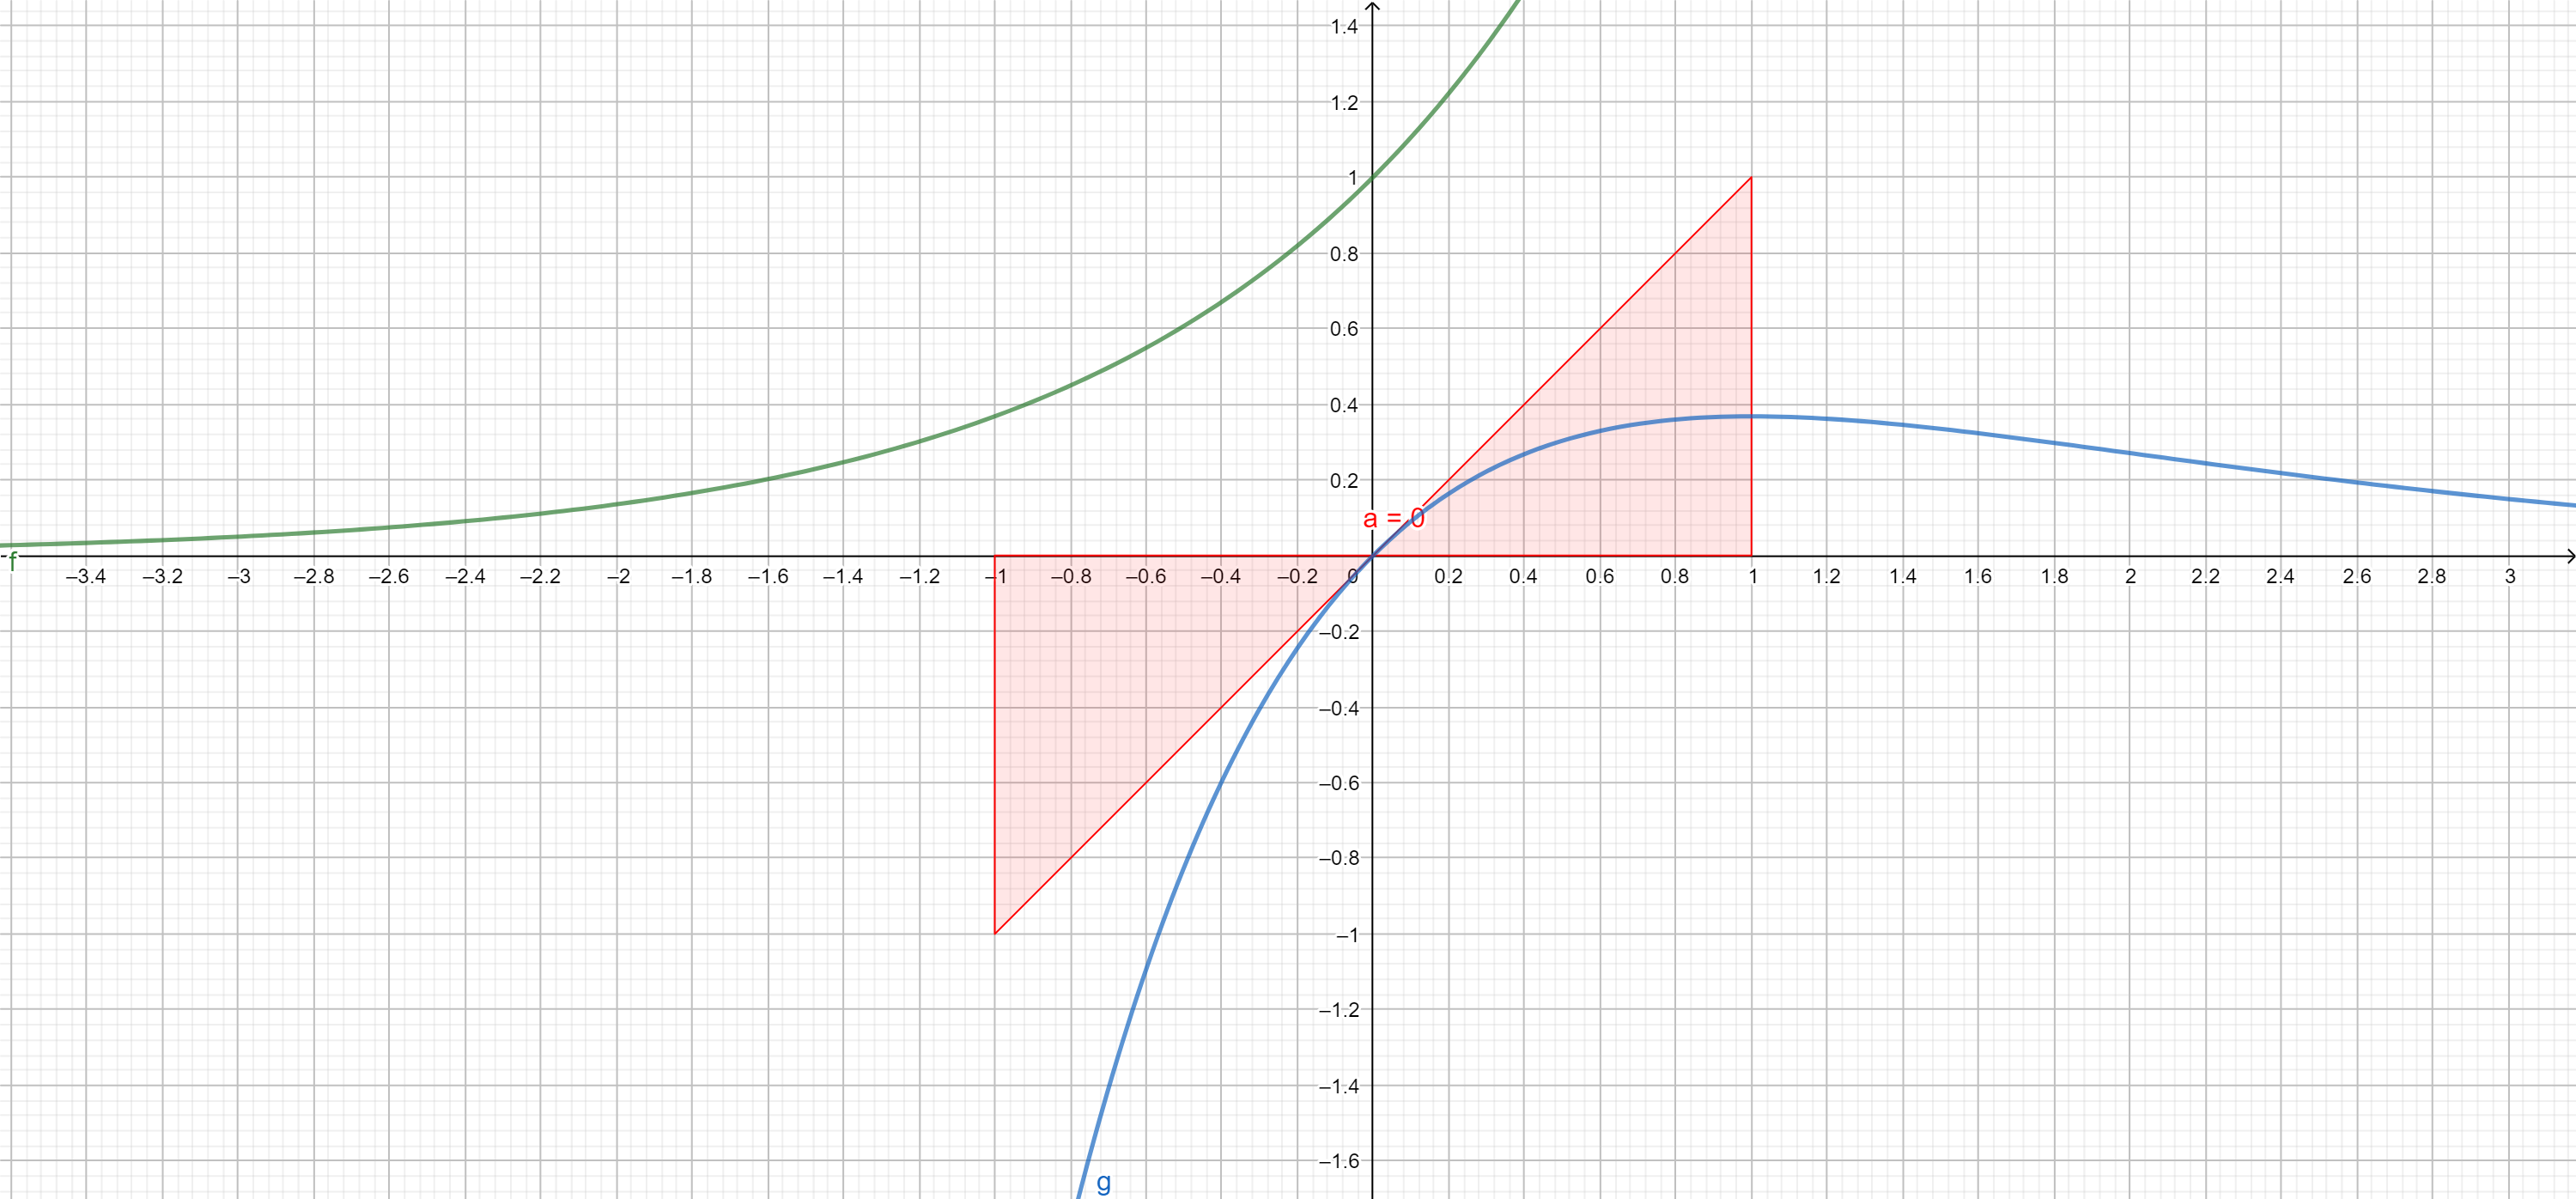
\includegraphics[width=.55\textwidth]{./img/inproduct functies.png}
    \caption{groen: f(x), blauw: g(x), rood: $\langle f,g\rangle$}
    \label{fig:my_label}
\end{figure}
We zeggen $x,y$ staan orthogonaal op elkaar  (in een Hilbertruimte) als $\langle x,y\rangle =0$.\\
De twee functies in het voorbeeld staan dus orthogonaal op elkaar. Functies die orthogonaal op elkaar staan hoeven elkaar dus niet loodrecht te snijden.

In een Hilbertruimte wordt de lengte van $x$ gegeven door $||x||=\sqrt{\langle x,x\rangle}$.

\textbf{Voorbeeld:} De lengte van $f(x)=-3ix^4+5x^2+10i$ is $\sqrt{\langle f,f\rangle}$.
\begin{align*}
    \langle f,f\rangle
    &= \int_{-1}^1 f(x)\overline{f(x)}  dx\\
    &= \int_{-1}^1 (-3ix^4+5x^2+10i)(3ix^4+5x^2-10i) dx\\
    &= \int_{-1}^1 9x^8+35x^4+100 dx\\
    &= \left[x^9+7x^5+100x\right]_{-1}^1=216
\end{align*}
Dus $||f||=\sqrt{216}$.

\begin{opdracht}
Laat het inproduct voor continue functies (die een reëel getal sturen naar een complex getal, bijvoorbeeld $e^{ix}$) gegeven zijn door $$\langle f,g\rangle=\int_{-1}^1 f(x)\overline{g(x)}dx.$$ met $\overline{g(x)}$ is de complex geconjugeerde van $g(x)$, bijvoorbeeld $\overline{e^{ix}}=e^{-ix}$.\\ Bereken $\langle f,g\rangle$.

\begin{enumerate}
    \item Bereken $\langle f,g\rangle$, \begin{align*}
        a.&\;& f(x)=x+4,g(x)=x^2+7\\
        b.&\;& f(x)=x^5+ix+7,g(x)=3x^3+2ix\\
        c.&\;& f(x)=\cos(x),g(x)=\tan(x)\\
        d.&\;& f(x)=e^{2\pi ix},g(x)=e^{4\pi ix}\\
    \end{align*}
%\end{enumerate}
%\end{opdracht}
%\begin{opdracht}
\item Gebruik hetzelfde inproduct als in de vorige opgave. Bereken $||f||$, \begin{align*}
        a.\;& f(x)=5x+1
        & c.\;& f(x)=6e^x\\
        b.\;& f(x)=2ix^3+4x+1
        & d.\;& f(x)=e^{2\pi ix}
    \end{align*}
\end{enumerate}
\end{opdracht}
\begin{opdracht}
Laat het inproduct voor 2-dimensionale reële vectoren gegeven zijn door $$\langle x,y\rangle=x_1y_1+(x_2-x_1)(y_2-y_1).$$
\begin{enumerate}

\item Wanneer geldt $x_1y_1+(x_2-x_1)(y_2-y_1)=x_1y_1+x_2y_2$. (geef een voorbeeld).
\item Bereken $\langle x,y\rangle$ voor $x=\begin{pmatrix}2\\1\end{pmatrix}$ en $y=\begin{pmatrix}-1\\-3\end{pmatrix}$, en concludeer dat ze orthogonaal op elkaar staan.
\item Laat zien dat $x$ en $y$ niet loodrecht op elkaar staan (hoek van $90^\circ$).
\end{enumerate}
\end{opdracht}

\textbf{Projectie:} In een Hilbertruimte wordt de projectie van $x$ op $y$ (allebei niet nul) gegeven door $\frac{\langle x,y\rangle}{\langle y,y\rangle}y$.

\begin{center}

%\hspace{-24pt}
%\begin{minipage}{\textwidth}
    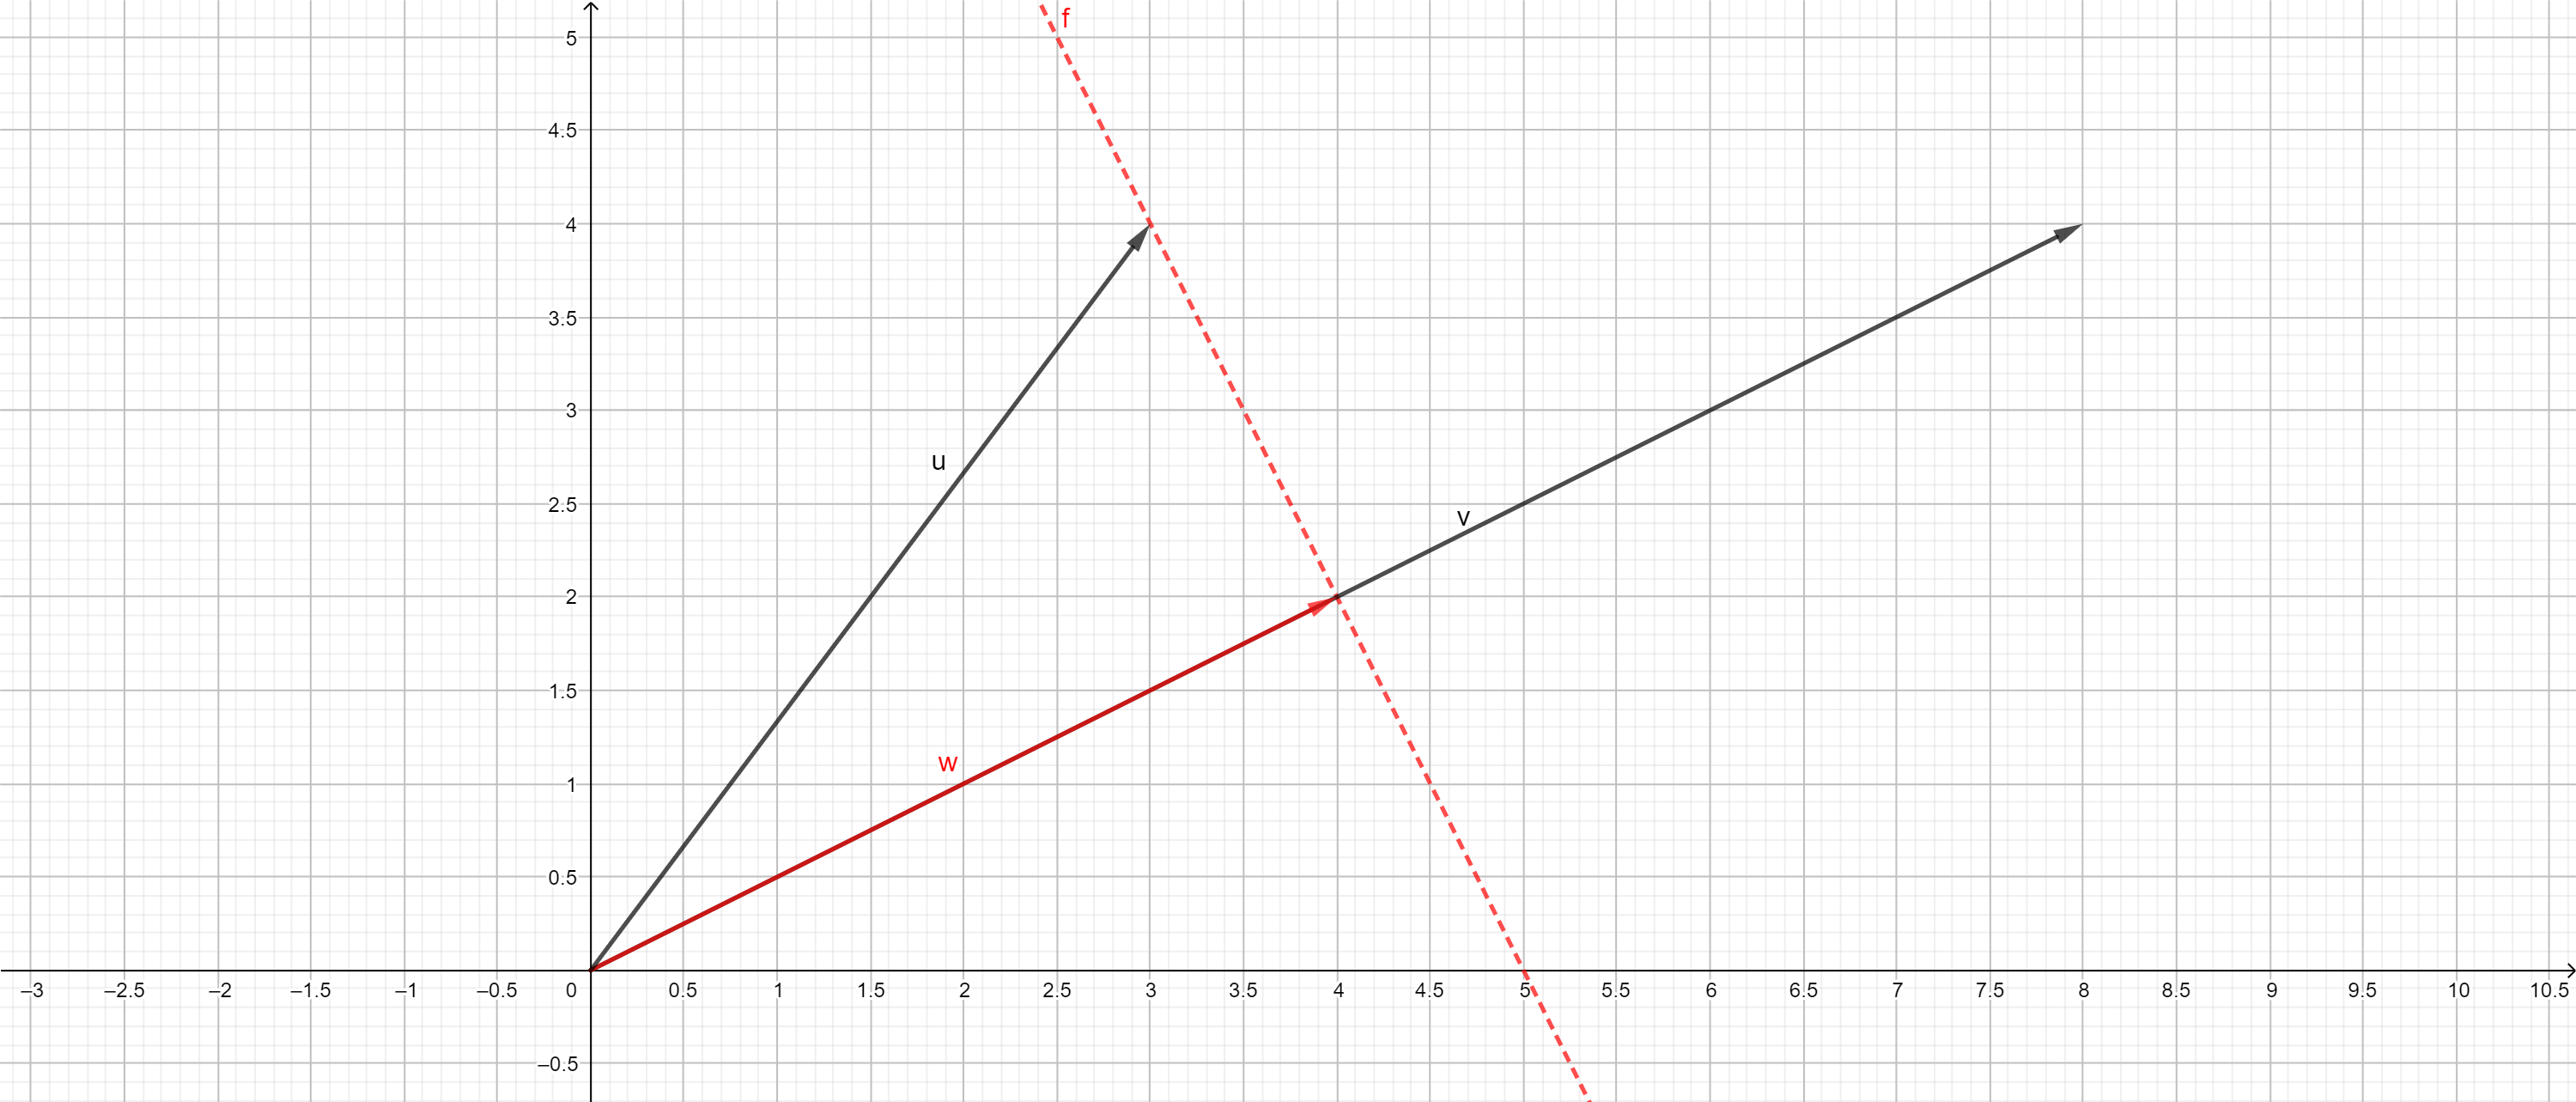
\includegraphics[width=0.55\textwidth]{./img/projectie 1.png}
%\end{minipage}
\captionof{figure}{$w$ is de projectie van $u$ op $v$ (met behulp van een loodlijn). \label{fig:fig:loodlijn}}
\end{center}
\vspace{.5cm}

Dus de projectie van $x$ op $y$ is altijd in de vorm $\lambda\cdot y$ met $\lambda$ een getal.

\begin{opdrachtlang}\label{opd:hilbproj}
\begin{enumerate}
\item Bereken de projectie (met het standaard inproduct) van $x=\begin{pmatrix}5\\2\end{pmatrix}$ op $y=\begin{pmatrix}1\\0\end{pmatrix}$ (dit is de projectie van $x$ op de $x$-as).\\
\item\label{itm:inprodb} Laat het inproduct voor reële functies \[\langle f,g\rangle=\int_{1}^2 f(x)g(x)dx\]\\
Laat $f(x)=\frac{e^x}{x},g(x)=x^3+4x^2$ en $h(x)=x$. Bereken de projectie van $f(x)$ op $h(x)$, en bereken de projectie van $g(x)$ op $h(x)$\\
\item Schets de functies gevonden bij~\ref{itm:inprodb}.\\
\item Laat zien dat de projectie van $x$ op $x$ gelijk is aan $x$. 
\end{enumerate}
\end{opdrachtlang}

\begin{opdrachtlang}
Stel je hebt $x$ en $y$ (met $x$ niet een veelvoud van $y$) dan kan je $z$ vinden zodat $z$ en $y$ orthogonaal op elkaar staan. Een manier om dit te doen is de projectie van $x$ op $y$ uitrekenen en die van $x$ aftrekken. Dit geeft de formule $z=x-\frac{\langle x,y\rangle}{\langle y,y\rangle}y$.

%\hspace{-24pt}
\begin{minipage}{\textwidth}
    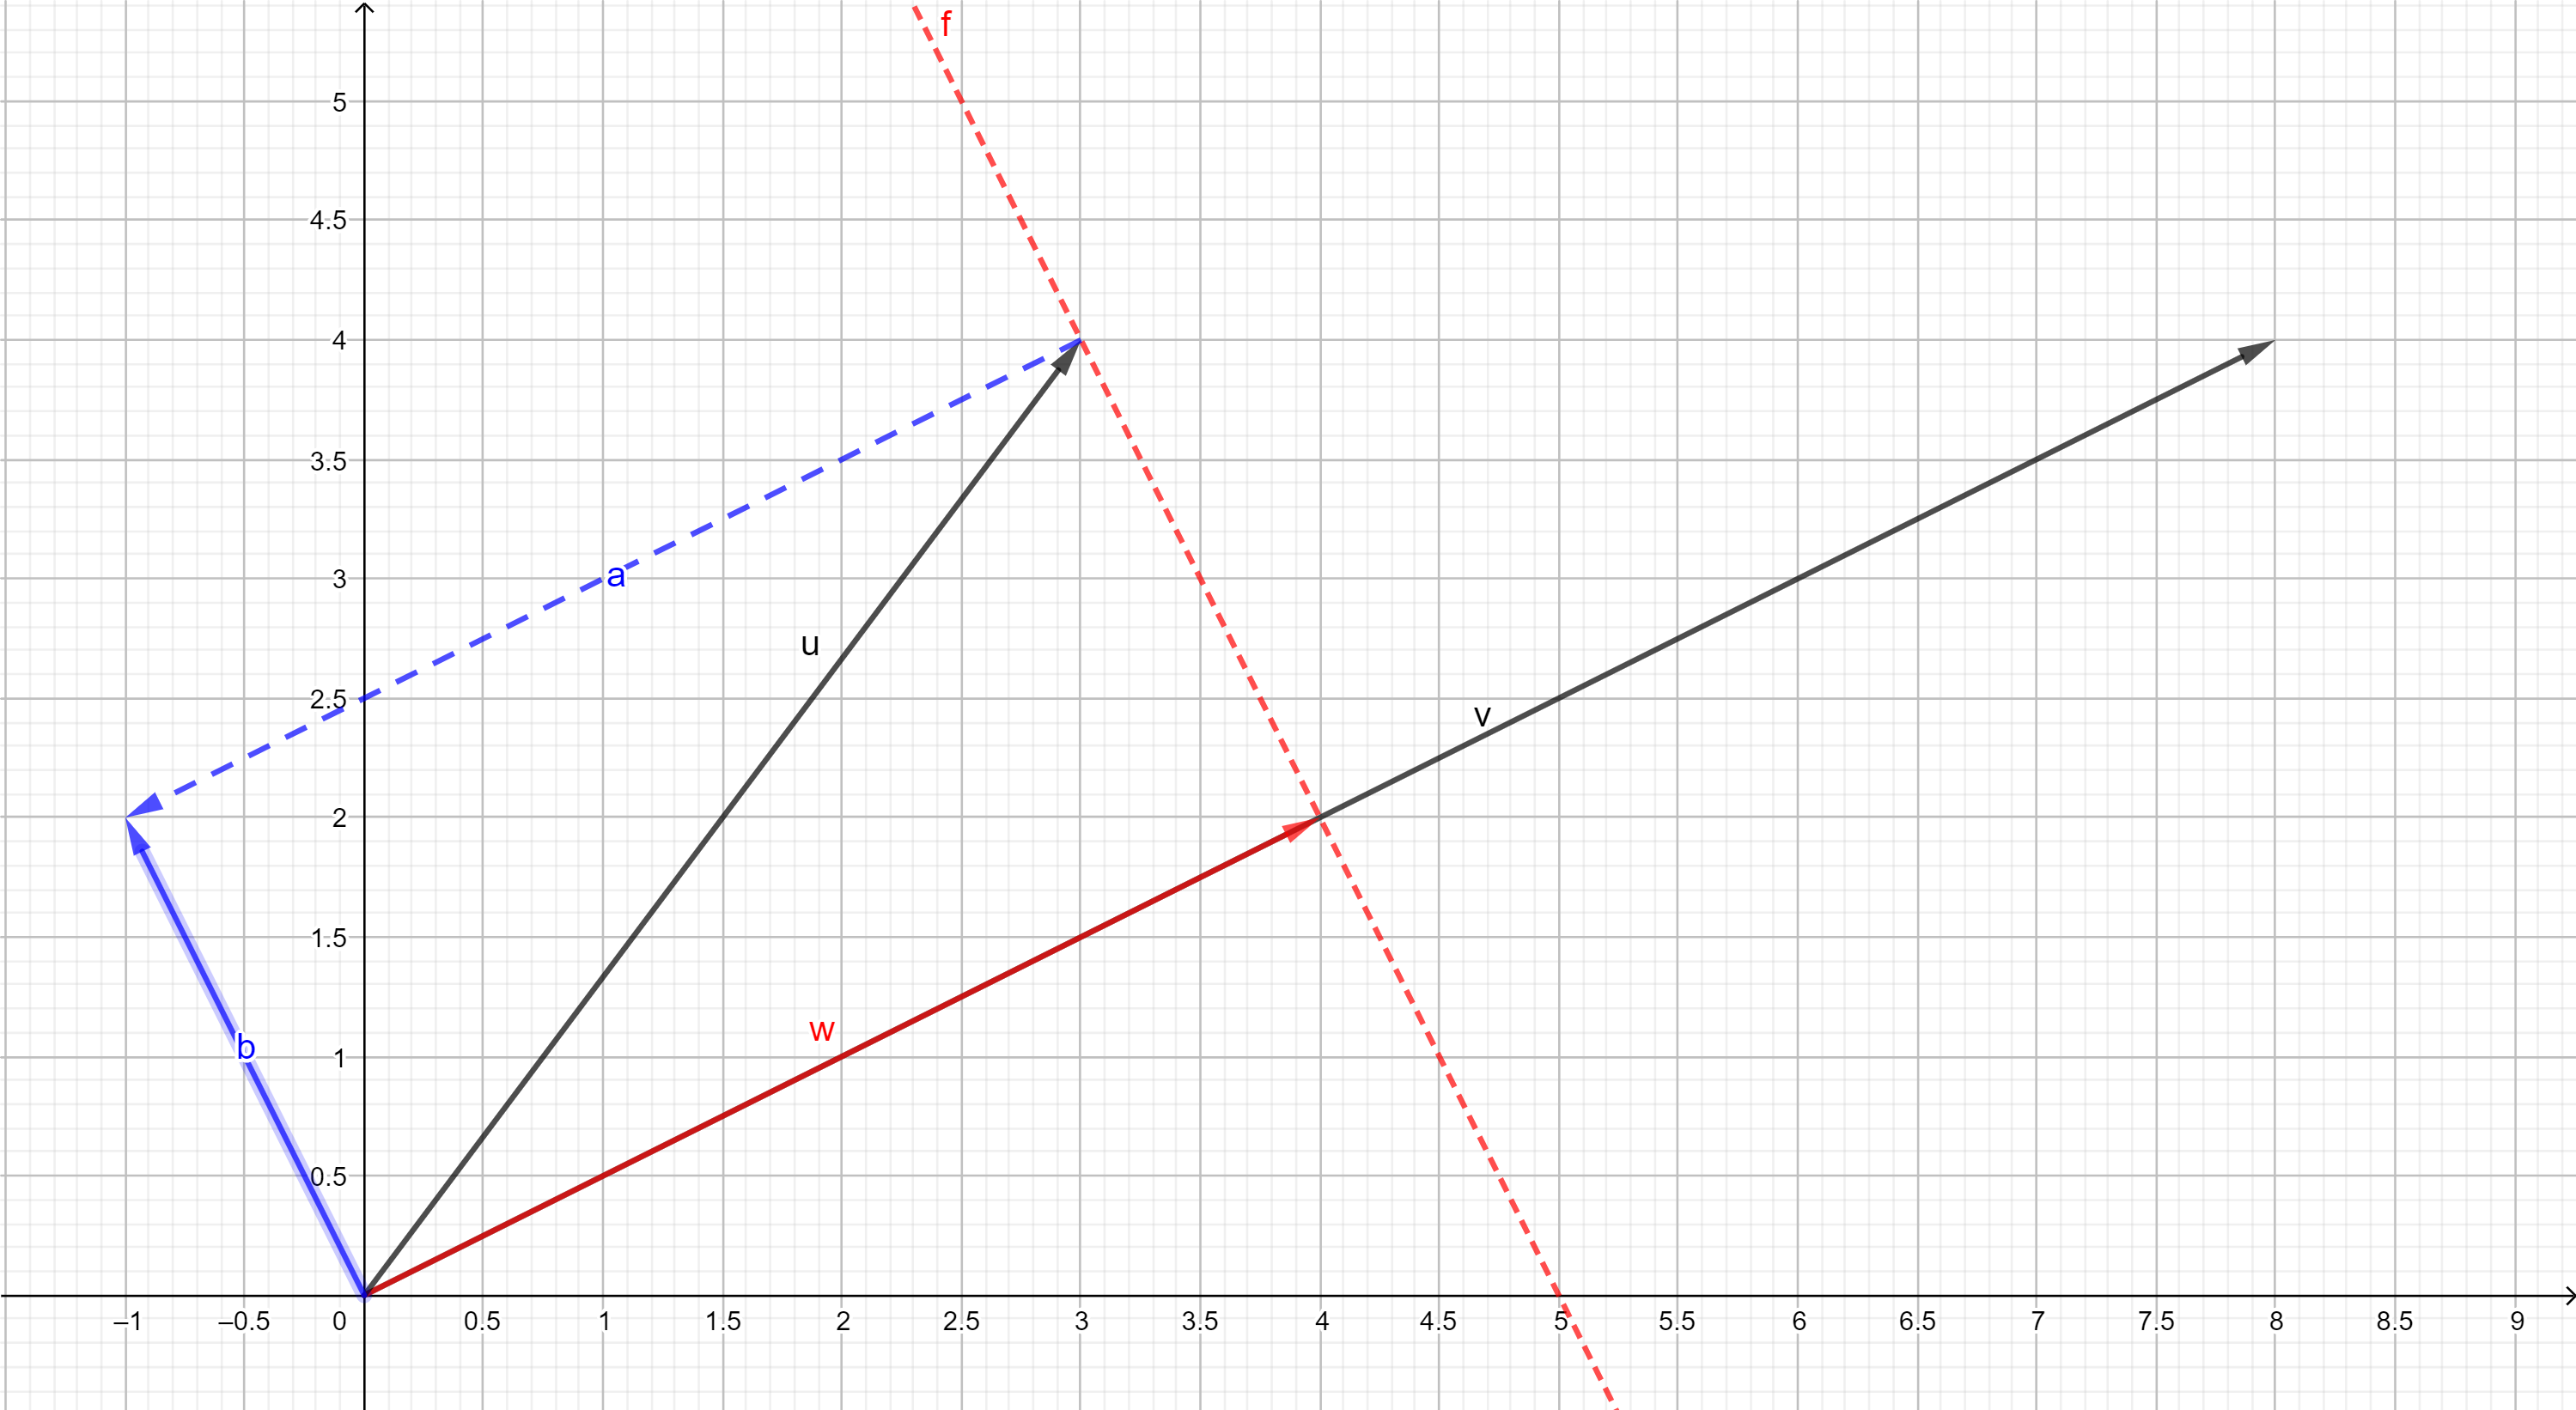
\includegraphics[width=.95\textwidth]{./img/projectie 2.png}
\end{minipage}
\captionof{figure}{b=u-w en inderdaad $b$ staat loodrecht op v. \label{fig:fig:projectie}}
\vspace{.5cm}


%    \begin{figure}[h]
%    \centering
%    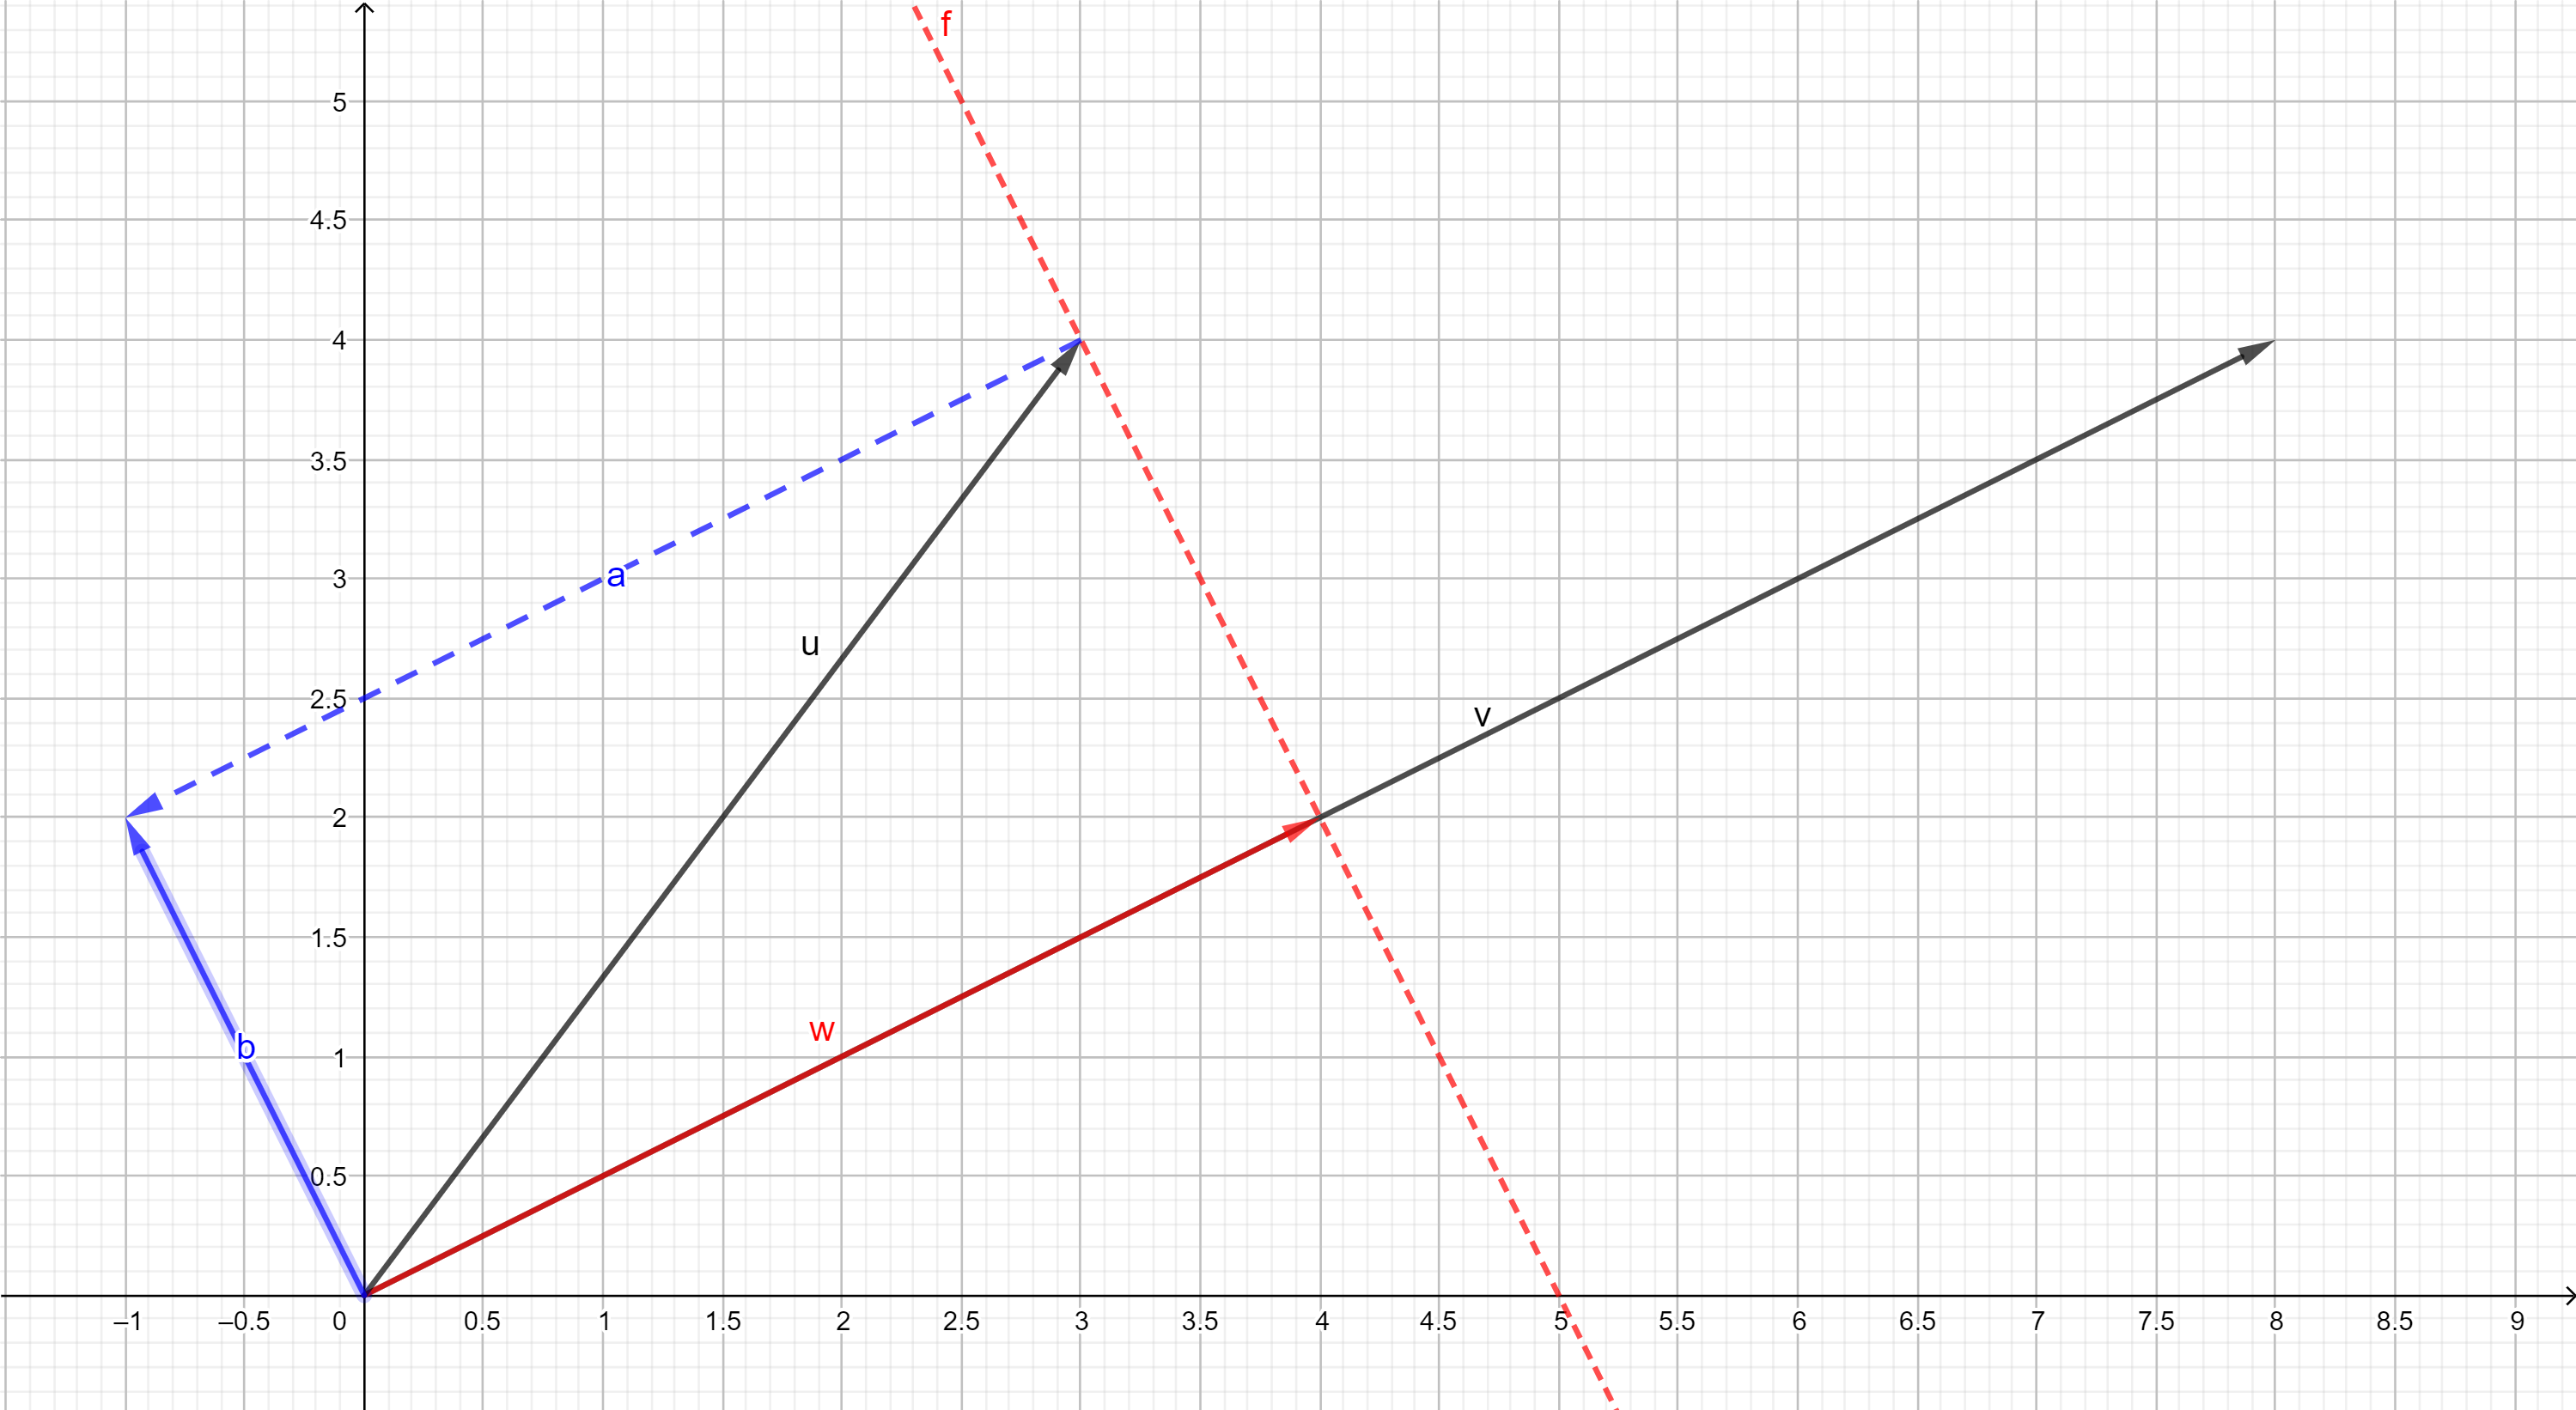
\includegraphics[scale=0.8]{./img/projectie 2.png}
%    \caption{b=u-w en inderdaad $b$ staat loodrecht op v}
%    \label{fig:my_label}
%\end{figure}


\begin{enumerate}
    \item Gebruik deze methode (met het standaard inproduct) om een orthogonaal element te vinden van $y=\begin{pmatrix}3\\1\end{pmatrix}$ met behulp van $x=\begin{pmatrix}7\\2\end{pmatrix}$. Ga na of de gevonden vector ook echt orthogonaal staat op $y$.
\item\label{itm:hilbfun} Laat het inproduct en de functies hetzelfde zijn als bij~\ref{itm:inprodb} van odracht~\ref{opd:hilbproj}. Vind twee functies die orthogonaal staan op $h$.\\
\item Schets de functies gevonden bij ~\ref{itm:hilbfun}.
\end{enumerate}
\end{opdrachtlang}

\begin{opdracht}
\textbf{Pythagoras:} We gaan in deze opgave laten zien dat de stelling van Pythagoras geldt in elke Hilbertruimte.
\begin{enumerate}
\item Laat zien dat voor elk inproduct geldt $\langle x,\lambda_1y+\lambda_2z\rangle=\overline{\lambda_1}\langle x,y\rangle+\overline{\lambda_2}\langle x,y\rangle$ met $\lambda_1,\lambda_2$ complexe getallen. (hint: $\overline{a+b}=\overline{a}+\overline{b}$)
\item Schrijf $||x+y||^2$ uit en concludeer $||x+y||^2=\langle x,x\rangle+\langle x,y\rangle + \langle y,x\rangle+\langle y,y\rangle$
\item Laat zien dat als $\langle x,y\rangle=\langle y,x\rangle =0$ (dus $x$ en $y$ orthogonaal op elkaar staan) dat dan  $||x+y||^2=||x||^2+||y||^2$ (de stelling van Pythagoras).
\end{enumerate}
\end{opdracht}
\nogdoen{afsluitende zinnen: waar heeft dit ons gebracht}
\section{Fourieranalyse}

In de quantumtheorie spelen golven een belangrijke rol. Fourieranalyse probeert functies te koppelen aan golven. Voor de sinus is dat natuurlijk niet moeilijk want dat is al een golf maar met Fourieranalyse kan je bijna alle functies zien als de som van golven, zelf functies zoals $\frac{1}{2}x$ kan je door maar een paar sinuso\"ides bij elkaar op te tellen erg goed benaderen. Ter voorbereiding hiervan zullen we eerst kijken naar een simpelere benaderingsmethode.

\subsection*{Taylorreeksen}
Zoals eerder gezegd kan je functies zien als vectoren (rijtjes getallen), in deze paragraaf laten we zien waarom dit zo is. We gaan proberen elke functie als een polynoom (bijvoorbeeld $x^4+3x^2+17$) te schrijven. Een voordeel hiervan is dat je door de eerste paar termen van het polynoom uit te rekenen je een zeer goede benadering krijgt van de functie (die makkelijk integreerbaar is). Voor een functie als $f(x)=x^9+5x^4+7$ is dat zeer makkelijk want dat is al een polynoom. We gaan het nu proberen $f(x)=e^x$ te schrijven als het polynoom $$g(x)=a_0+a_1x+a_2x^2+a_3x^3+\ldots$$ Omdat $f(x)=g(x)$ en $f(0)=1$ geldt $g(0)=a_0=1$. Om $a_1$ uit te rekenen is het niet handig om een ander punt invullen want $$g(1)=a_0+a_1+a_2+\ldots$$ dit geeft geen makkelijke manier om $a_1$ uit te rekenen. Dus we gebruiken de afgeleide $f'(x)=e^x$ dus $f'(0)=1$ maar $$g'(x)=a_1+2a_2x+3a_3x^2+4a_4x^3$$
dus $g'(0)=a_1=1$. Op dezelfde manier kan je door de afgeleide van $f'(x)$ (dus $f''(x)$) gebruiken om $a_2=\frac{1}{2}$ te vinden. Als je de eerste 6 termen uitrekent krijg je: $$g(x)=1+x+\frac{1}{2}x^2+\frac{1}{6}x^3+\frac{1}{24}x^4+\frac{1}{120}x^5$$
\begin{figure}[h]
    \centering
    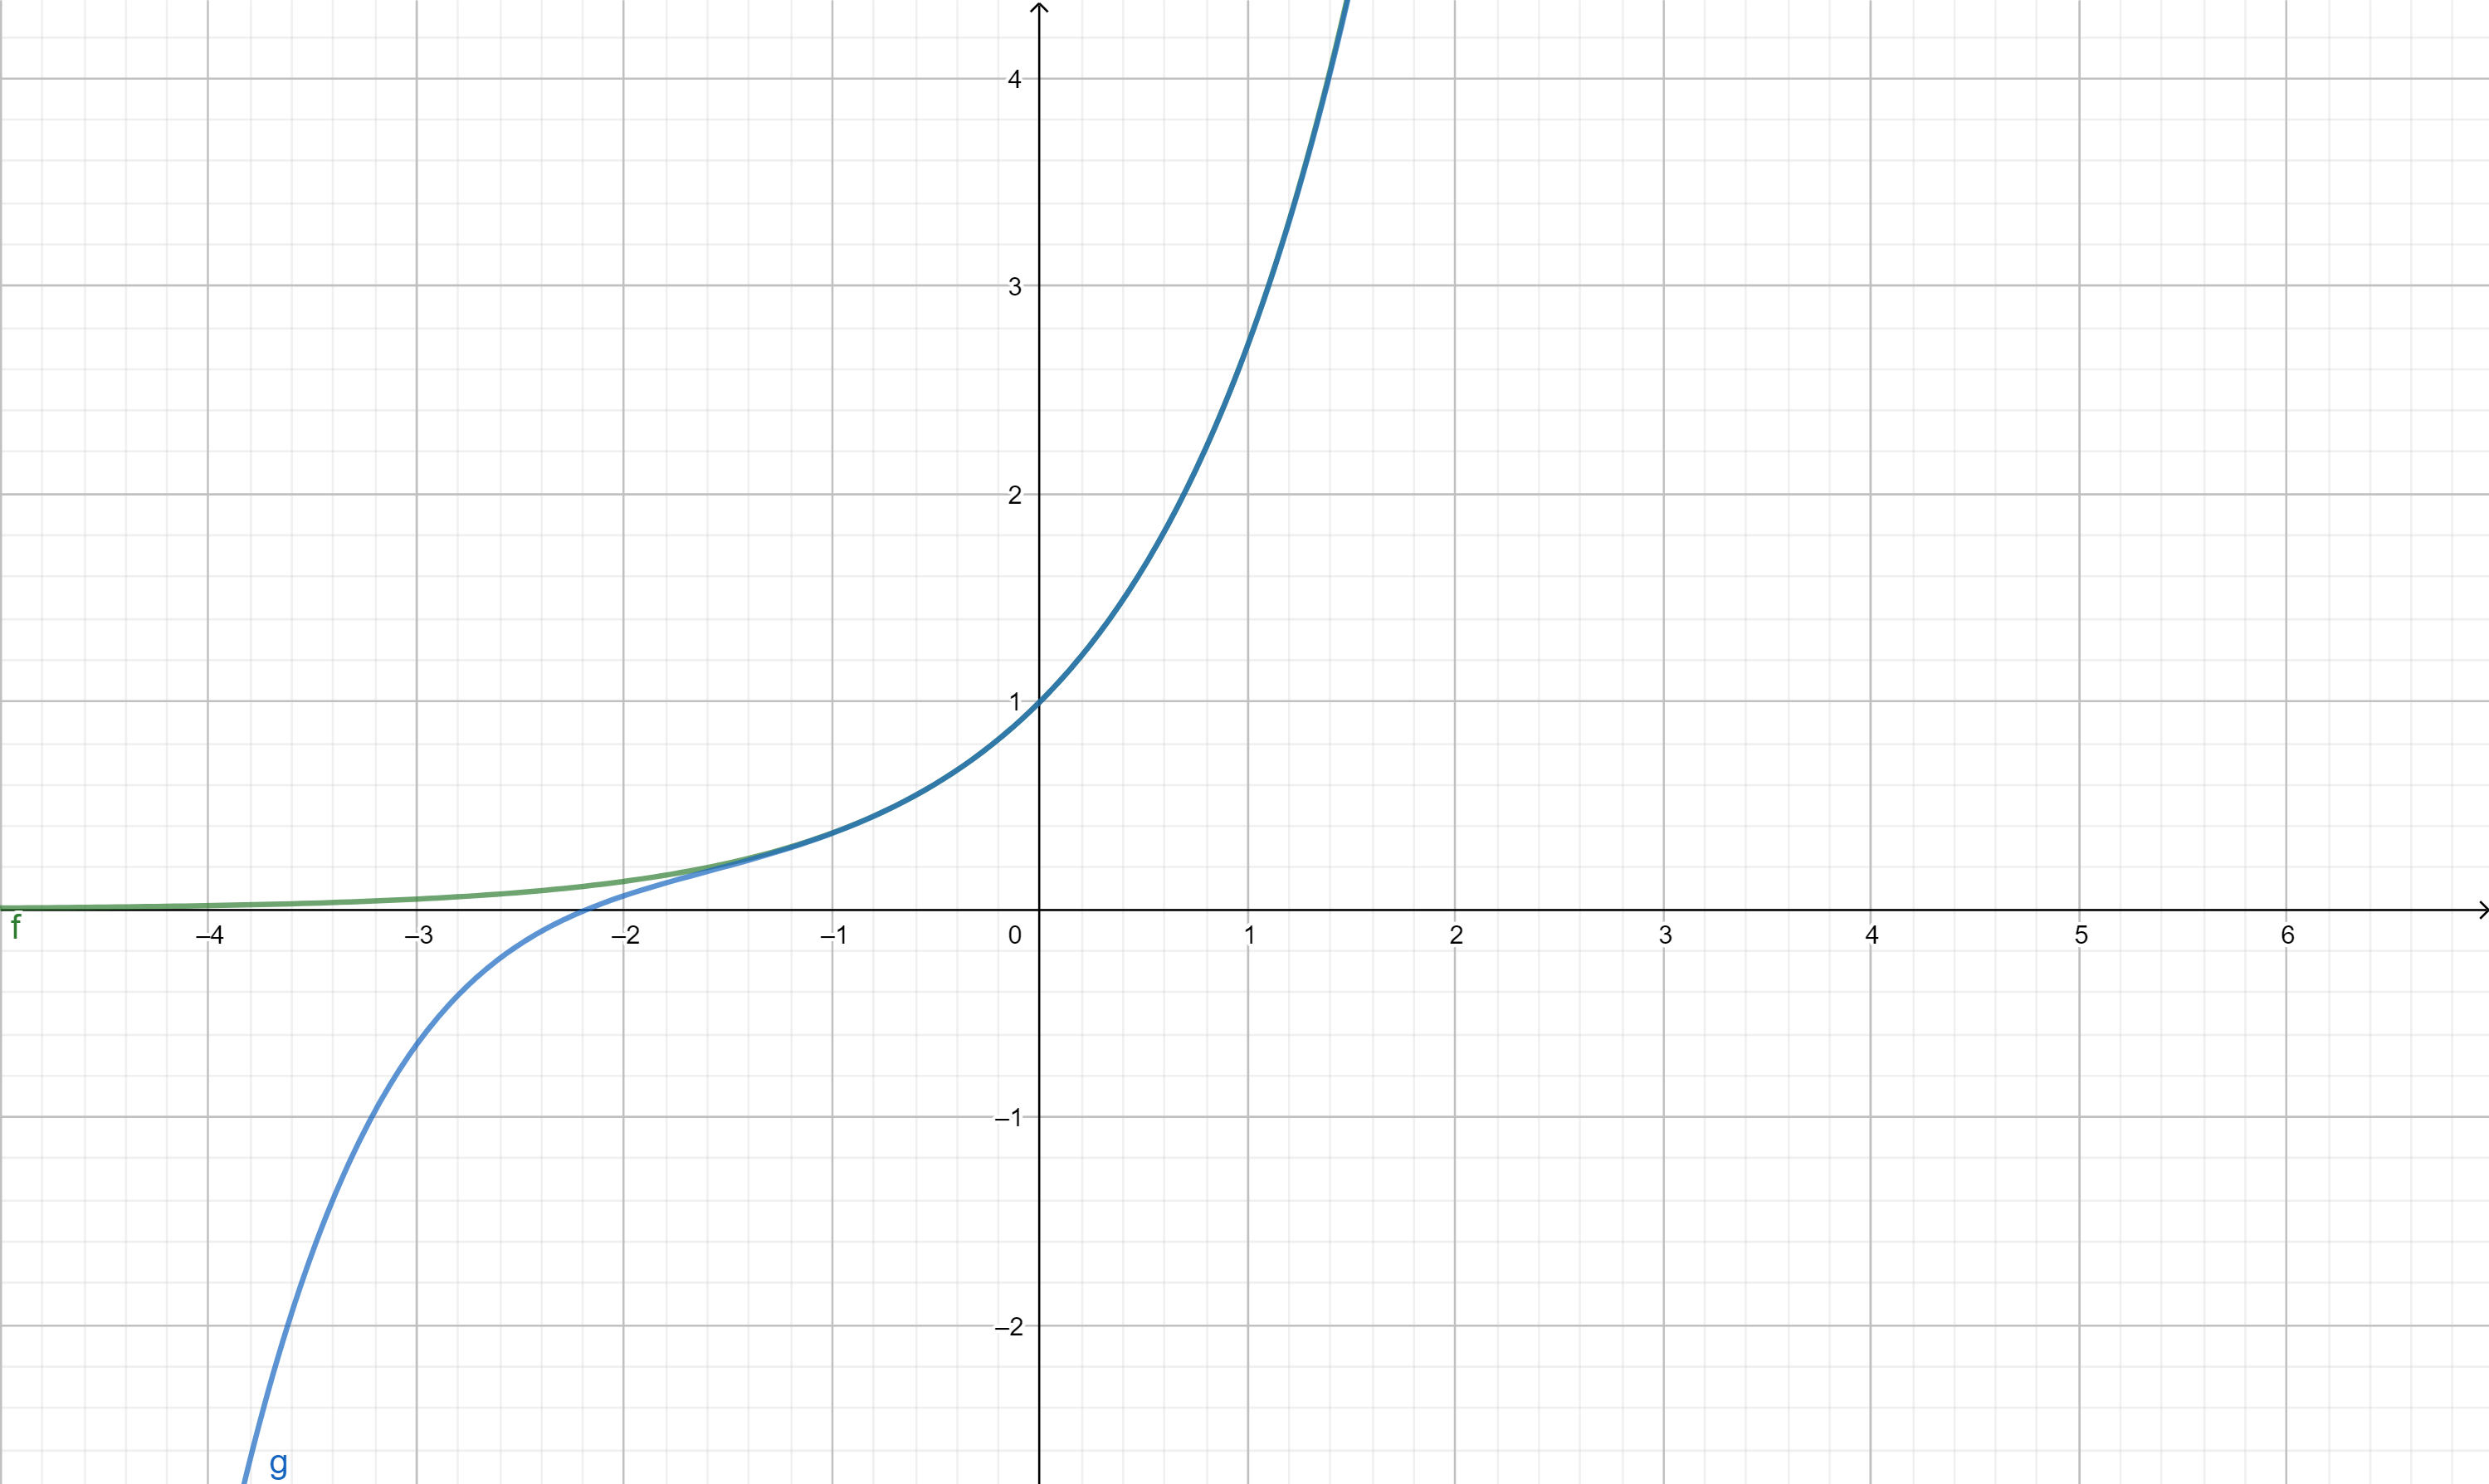
\includegraphics[width=.55\textwidth]{./img/taylor.png}
    \label{fig:my_label}
\end{figure}

Je ziet rond 0 dat $g$ een goede benadering is van $f$, als je meer termen toevoegt zal de benadering steeds beter worden en als je oneindig veel termen hebt zijn $g$ en $f$ gelijk.\\
De algemene formule van een Taylorreeks (rond 0) voor een functie $f$ is $$g(x)=f(0)+f^{(1)}(0)x+\frac{f^{(2)}(0)}{2!}x^2+\frac{f^{(3)}(0)}{3!}x^3+\frac{f^{(4)}(0)}{4!}x^4+\ldots$$
Hierbij is $f^{(n)}(0)$ de $n-$de afgeleide in 0 dus $f^{(2)}(0)=f''(0)$ en $n!=1\cdot2\cdot3\cdot\ldots\cdot n$ dus $4!=1\cdot2\cdot3\cdot4=24$ ($0!=1$).\\
We bekijken weer $f(x)=e^x$ omdat ook $f'(x)=e^x$ geldt $f^{(n)}(0)=e^0=1$ dus $$g(0)=1+x+\frac{1}{2!}x^2+\frac{1}{3!}x^3+\frac{1}{4!}x^4+\ldots$$
Je kan dus $e^x$ zien als de rij getallen $(1,\frac{1}{2!},\frac{1}{3!},\frac{1}{4!},\ldots)$.

\begin{opdracht}
\begin{enumerate}
    \item Bereken de eerste 4 termen van de Taylorreeks van de volgende functies en plot $f$ en $g$

     \begin{align*}
        a.\;& f(x)=x^5+2x^4+3x^2+12x+3
        & c.\;& f(x)=2e^{2x}\\
        b.\;& f(x)=\sin(x)
        & d.\;& f(x)=e^{x^2}
    \end{align*}
\end{enumerate}
Als je een Taylorreeks probeert te maken van $f(x)=\frac{1}{x}$ heb je een probleem want $f(0)$ is niet gedefinieerd.
\begin{enumerate}[resume]
    \item Vervang $x$ door $x=y+1$ en bereken $f^{(1)}(y),f^{(2)}(y)$ en $f^{(3)}(y)$.
    \item Bepaal de eerste 4~termen van de Taylorreeks van $f(y)$.\\
    \item Substitueer $y=x-1$ in de Taylorreeks en plot $f$ en $g$\\
    \item Gebruik de zelfde truc om een benadering te maken (4~termen) van $f(x)=\ln(x)$.
\end{enumerate}
\end{opdracht}

\subsection*{Fourierreeksen}
In deze paragraaf gaan we een andere benadering vinden van (periodieke) functies aan de hand van sinusoïde. Hiervoor gebruiken we het volgende inproduct: \[\langle f,g\rangle=\frac{1}{2\pi}\int_{0}^{2\pi} f(x)g(x)dx.\]
Als benadering voor de functie $f$ gebruiken we nu de volgende functie 
\begin{align*}
    g(x)=&a\\
    &+b_1\sin(x)+b_2\sin(2x)+b_3\sin(3x)+\ldots\\
    &+c_1\cos(x)+c_2\cos(2x)+c_3\cos(3x)+\ldots
\end{align*}
Als we proberen $a$ uit te rekenen (op dezelfde manier zoals bij Taylorreeksen) komen we in de problemen want als $\sin(x)=0$ dan $\cos(x)\neq 0$. 
Daarom gebruiken we dat als $f=g$ dat dan de projectie $P$ op $h(x)=1$ voor $f$ en $g$ hetzelfde zijn.
\begin{align*}
    P(x)&=\frac{\langle g,h\rangle}{\langle h,h\rangle}h\\
    &=\langle a,h\rangle+\langle b_1\sin(x),h\rangle+\langle c_1\cos(x),h\rangle+\ldots
\end{align*}
maar omdat $h(x)=\cos(0x)$ is $h$ een sinusoïde dus staat $h$ orthogonaal op alle andere sinusoïde. Dus\\
\begin{align*}
    P(x)&=\langle a,h\rangle\\
    &=\frac{1}{2\pi}\int_0^{2\pi}adx=a
\end{align*}
Ook geldt \begin{align*}
    P(x)&=\frac{\langle f,h\rangle}{\langle h,h\rangle}h\\
    &=\frac{1}{2\pi}\int_0^{2\pi}f(x)dx
\end{align*}
Dus $$a=\frac{1}{2\pi}\int_0^{2\pi}f(x)dx=\langle f,1\rangle$$.\\
Op dezelfde manier geldt\begin{align*}
     b_n&=\frac{1}{\pi}\int_0^{2\pi}f(x)\sin(nx)dx=2\langle f,\sin(nx)\rangle\\ c_n&=\frac{1}{\pi}\int_0^{2\pi}f(x)\cos(nx)dx=2\langle f,\cos(nx)\rangle.\\
     \end{align*}
Als voorbeeld bekijken we $f(x)=\frac{1}{2}x$ dan geldt 
\begin{align*}
    a&=\frac{1}{2\pi}\int_0^{2\pi}\frac{1}{2}xdx=\frac{1}{2\pi}\left[\frac{1}{4}x^2\right]_0^{2\pi}=\frac{\pi}{2}\\
    b_1&=\frac{1}{\pi}\int_0^{2\pi}\frac{1}{2}x\sin(x)dx=\frac{1}{\pi}\left[\frac{1}{2}\sin(x)-\frac{1}{2}x\cos(x)\right]_0^{2\pi}=-1\\
    c_1&=\frac{1}{\pi}\int_0^{2\pi}\frac{1}{2}x\cos(x)dx=\frac{1}{\pi}\left[\frac{1}{2}x\sin(x)+\frac{1}{2}\cos(x)\right]_0^{2\pi}=0
\end{align*}
Dus we krijgen als benadering $g(x)=\frac{\pi}{2}-\sin(x)$.
\begin{figure}[h]
    \centering
    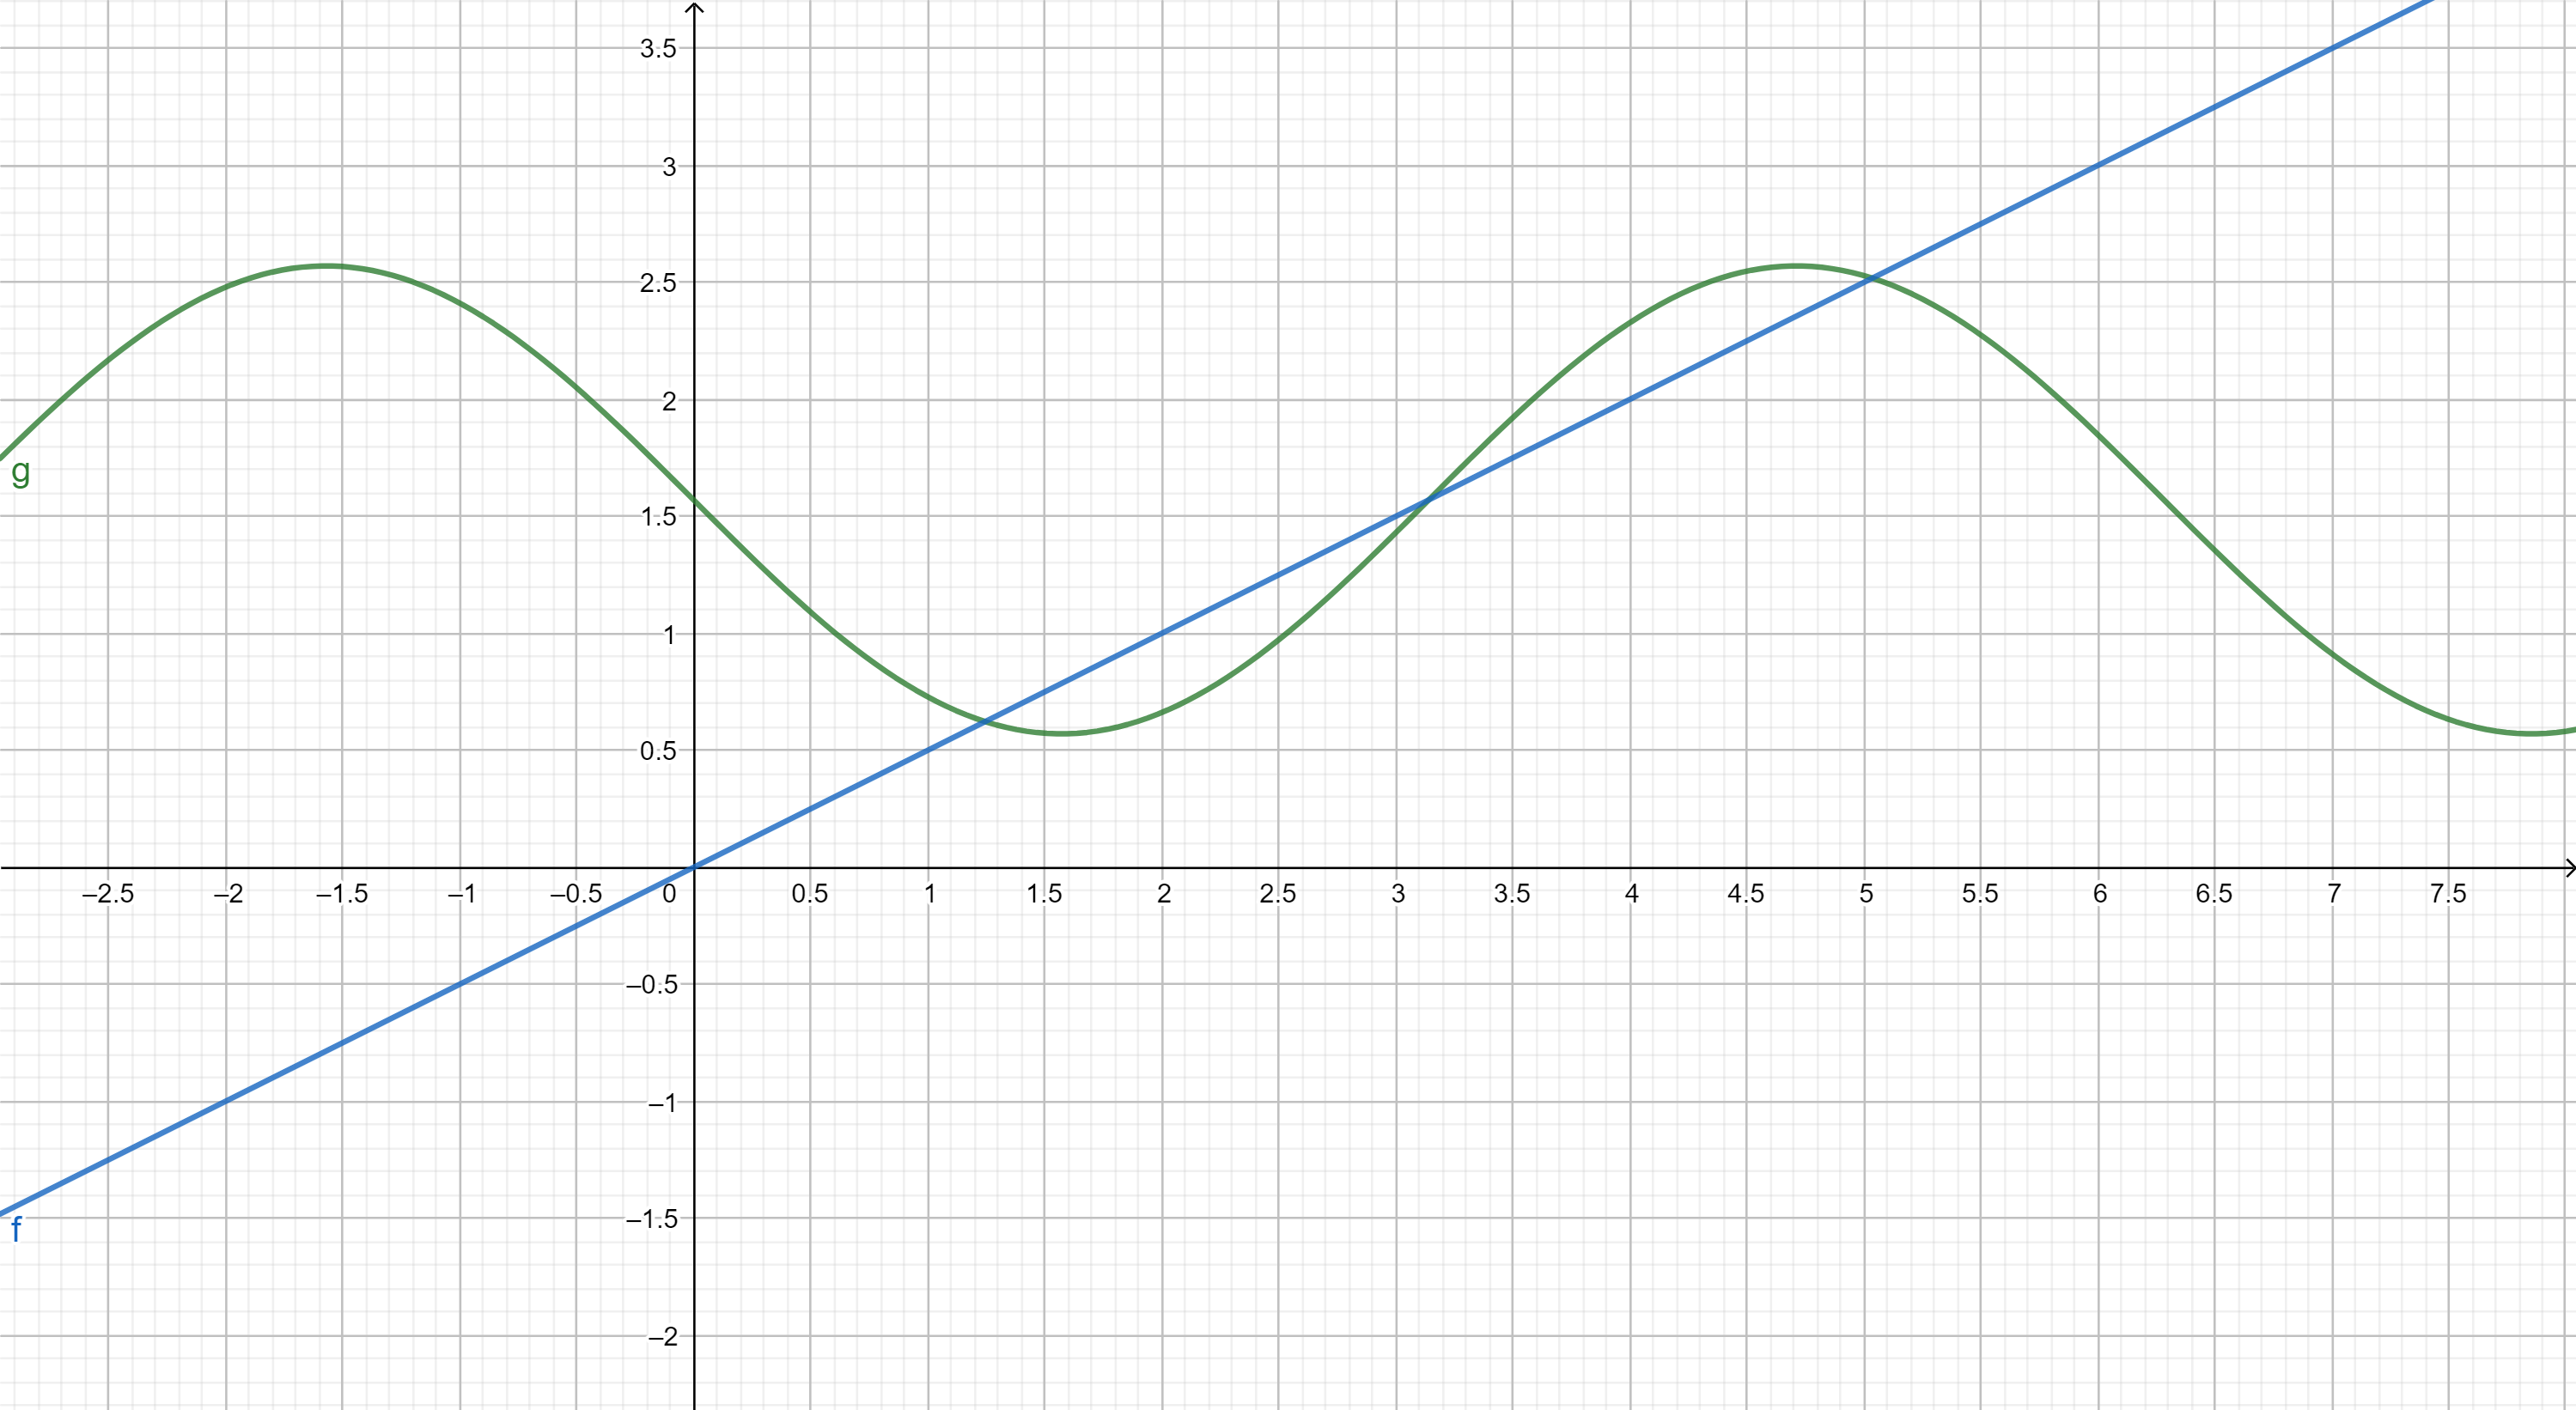
\includegraphics[width=.55\textwidth]{./img/fourier_1.png}
    \label{fig:my_label}
\end{figure}

Zoals je ziet is het nog niet zo 'n goede benadering. Als je $b_2$ tot en met $b_5$ \ en $c_2$ tot en met $c_5$ uitrekent krijg je $$g(x)=\frac{\pi}{2}-\sin(x)-\frac{1}{2}\sin(2x)-\frac{1}{3}\sin(3x)-\frac{1}{4}\sin(4x)-\frac{1}{5}\sin(5x)$$
\begin{figure}[h]
    \centering
    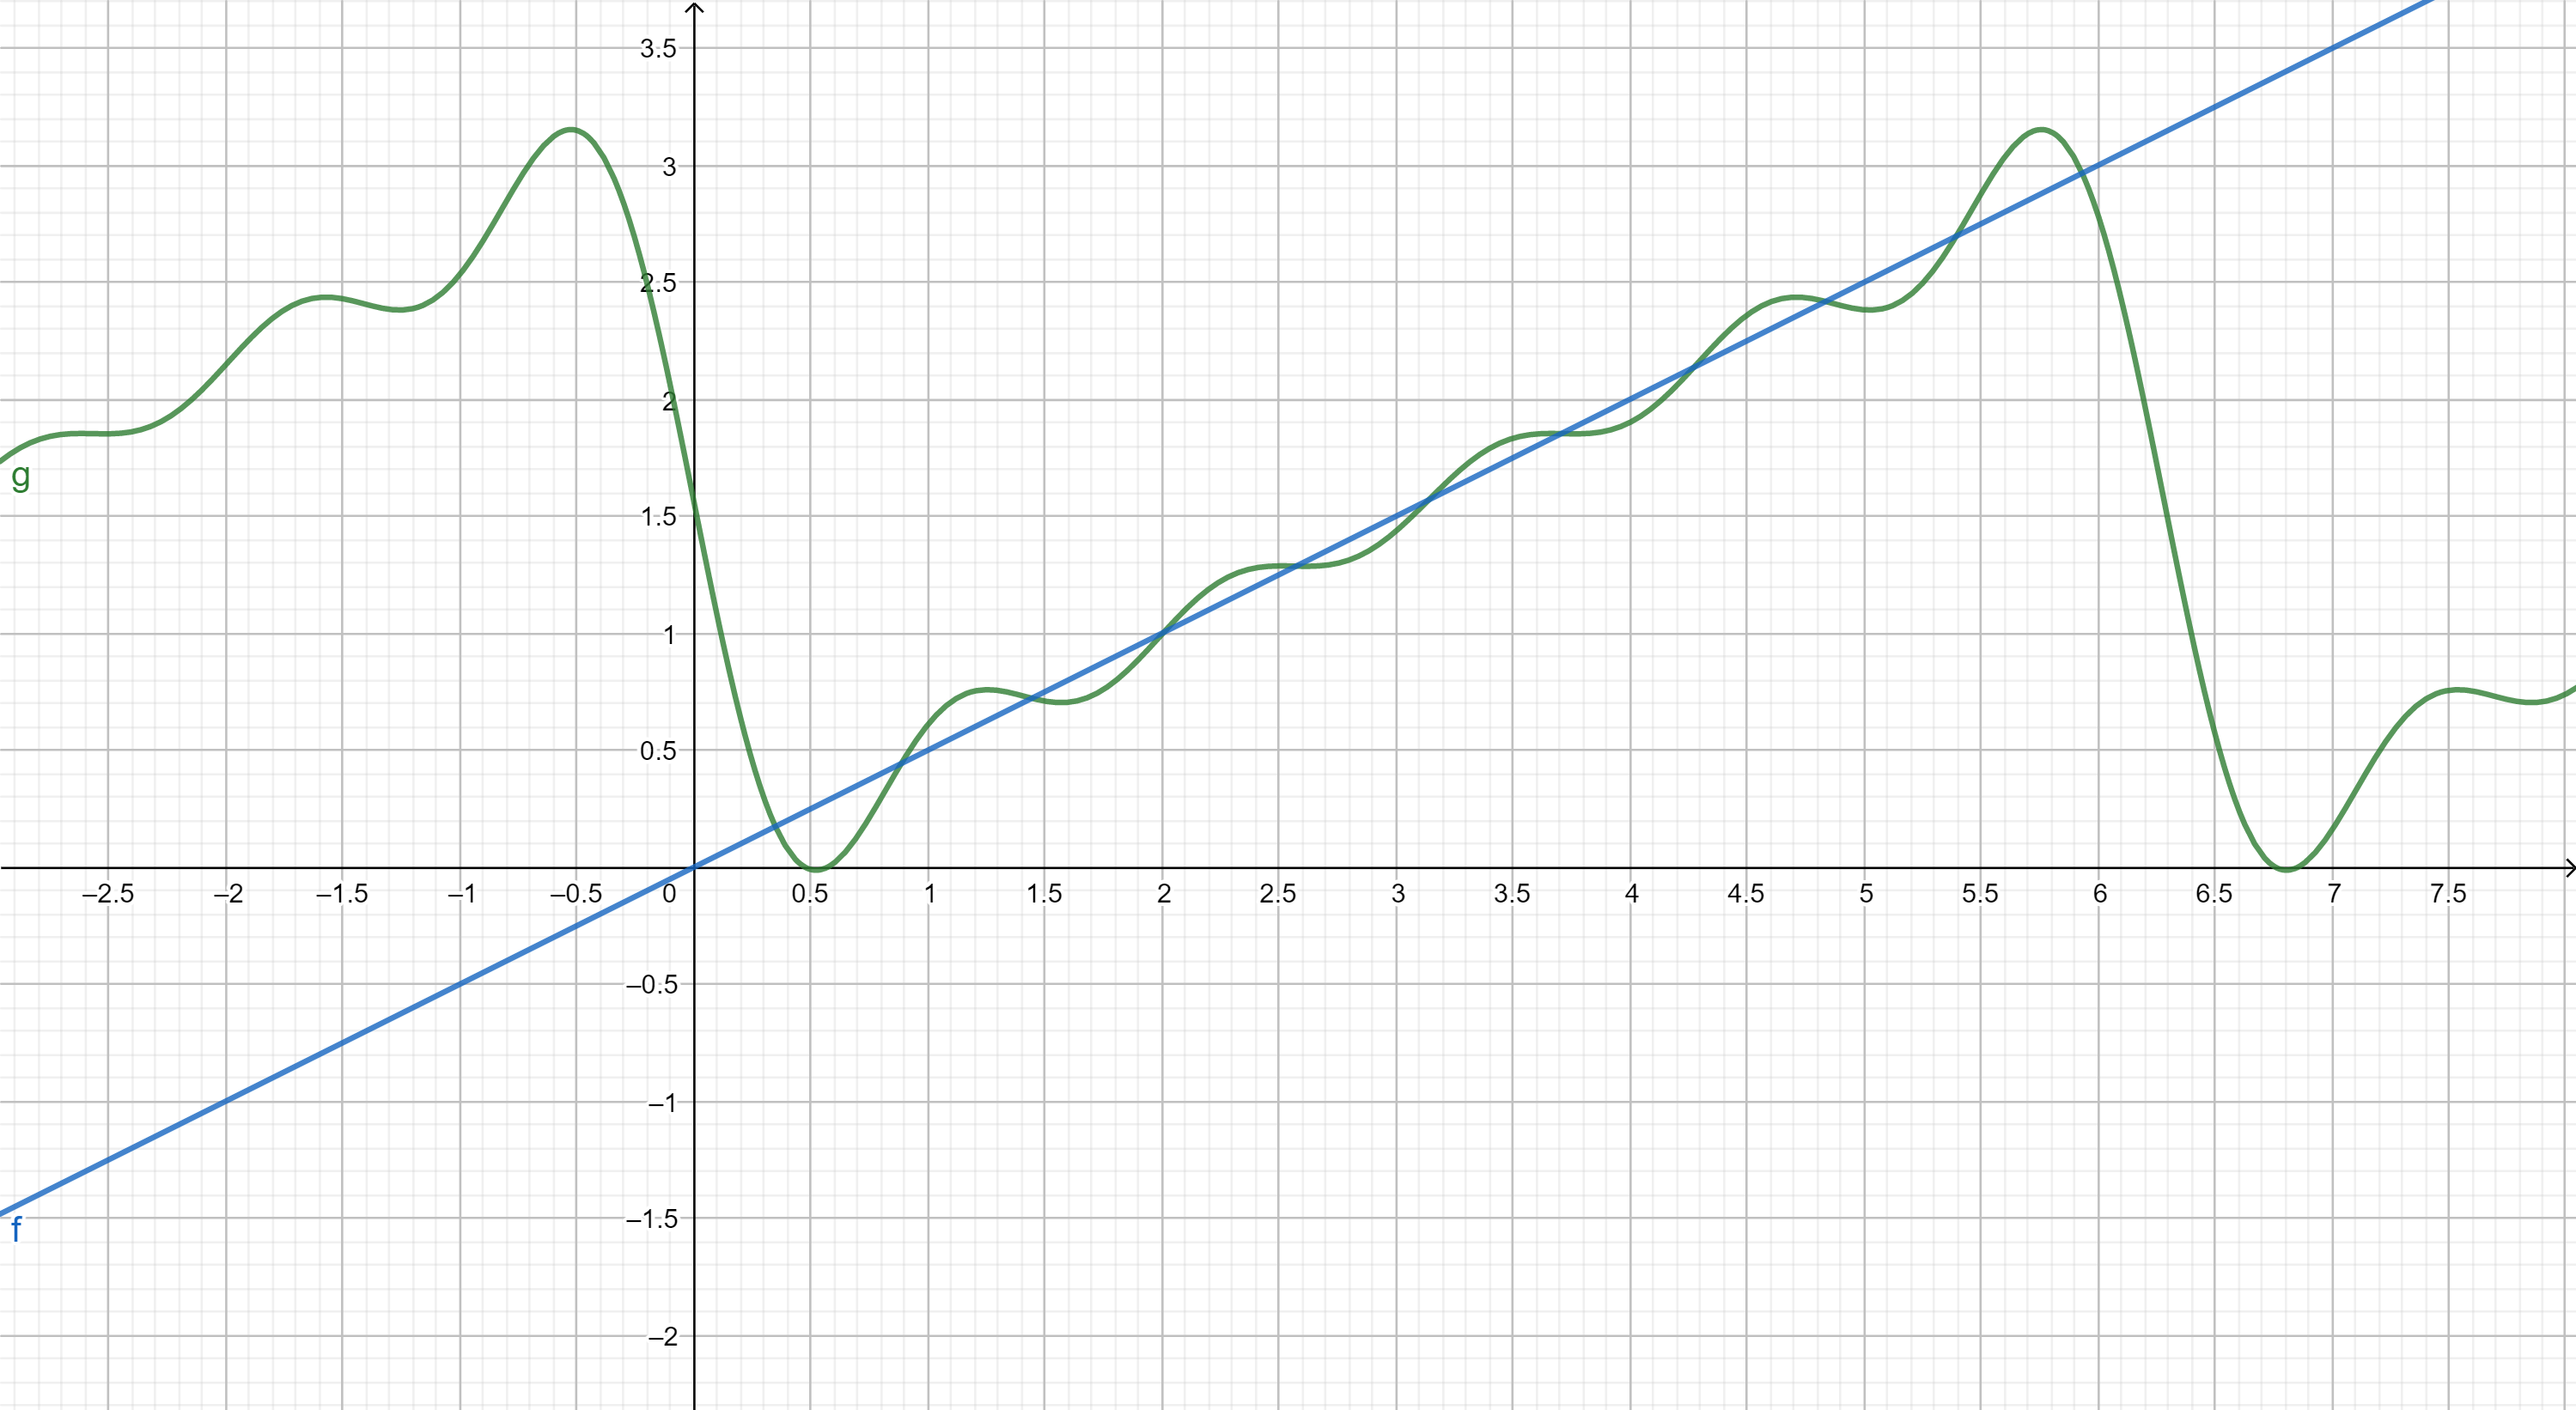
\includegraphics[width=.55\textwidth]{./img/fourier_2.png}
    \label{fig:my_label}
\end{figure}

Dit is al een veel betere benadering, maar alleen in het interval $(0,2\pi)$ daarna herhaalt de grafiek zich. Dit blijft het geval hoeveel termen je ook uitrekent daarom is deze manier juist geschrikt voor herhalende functies.

\begin{opdrachtlang}
\begin{enumerate}
    \item a. Laat zien $\int \sin(2x)\cos(x) dx=-\frac{2}{3}\cos^3(x)$.\\
    b. Laat zien dat $\sin(2x)$ en $\cos(x)$ orthogonaal op elkaar staan (met het hierboven genoemde inproduct).
    \item Bereken $a, b_1,b_2,c_1$ en $c_2$ van de Fourierreeks van de volgende functies (met behulp van je GR) en plot $f$ en $g$. \begin{align*}
        a.\;& f(x)=x^2-x-1
        & c.\;& f(x)=e^{x}\\
        b.\;& f(x)=\tan(\frac{x-\pi}{2})
        & d.\;& f(x)=\frac{1}{x+1}
    \end{align*}
\end{enumerate}

We kunnen ook een ander inproduct nemen voor een fourierreeks. Beschouw \[\langle f,g\rangle=\frac{1}{4\pi}\int_{-2\pi}^{2\pi} f(x)g(x)dx\]

Net als hiervoor zoeken we een benadering voor een functie $f$ en die benadering is nog steeds
    \begin{align*}
        g(x)=&a\\
        &+b_1\sin(x)+b_2\sin(2x)+b_3\sin(3x)+\ldots\\
        &+c_1\cos(x)+c_2\cos(2x)+c_3\cos(3x)+\ldots
    \end{align*}
\begin{enumerate}[resume]
\item Laat zien met behulp van projectie dat $a=\langle f,1\rangle$.
\end{enumerate}

Er geldt $b_n=\langle f,\sin(nx)\rangle$ en $c_n=\langle f,\cos(nx)\rangle$. 
\begin{enumerate}[resume]
\item Bereken $a, b_1,b_2,c_1$ en $c_2$ van de Fourierreeks van de volgende functies (met behulp van je GR) en vergelijk met de antwoorden gevonden bij opgave $2$.
   \begin{align*}
a.\;& f(x)=x^2-x-1.\\
b.\;& f(x)=e^x.\\
    \end{align*}
    
\end{enumerate}
\end{opdrachtlang}
\nogdoen{afsluitende zinnen waar heeft dit ons gebracht?}
\iffalse%-----------
\fi%---------------------
\end{document}